%!TEX root = predictability.tex

\section{Introduction}
\label{sec:intro}

Transactional databases are a key component of almost every enterprise software, where 
mission-critical applications rely on the underlying DBMS to store and manipulate data efficiently and reliably. 
Consequently, a significant portion of database research on transactions has focused on reducing latency and 
increasing  throughput, e.g.,  through
 concurrency control and recovery protocols, query optimization techniques, indexing schemes, 
 caching policies, \tofix{and many other sophisticated ideas.} 
These strategies, however, have been mostly evaluated  in terms of
 their effect on the \emph{average performance} of a transactional database, such as its throughput 
 or mean latency in executing transactions. 
 In other words, the focus has often been on running more and/or faster transactions \emph{overall}.
The effect of these strategies on the spread of the latency distribution has largely remained unvetted.
\tofix{Have our traditional database design principles sacrificed the tail latencies for the sake of improving average performance
of transactions? 
Do our existing databases exhibit a notable latency variance in practice?
If so, how much of this variance is due to 
our database implementation and how much of it is due to the 
the variations in the user's queries themselves?
How can we measure the contribution of each component/algorithm 
of our database to 
 the overall latency variance?
And most importantly,  do we need to compromise on the mean latency to reduce its variance or $99\%$ quantile, and if so, how?}

%ta inja 

We believe that it is critical and particularly timely to ask these questions. 
First, the past four decades of research on transactions has matured to a point where  
microsecond latencies and hundreds of thousands of concurrent transactions are now 
achievable \cite{??}.\tempcut{\footnote{Human-triggered transactions are bound by human population, and hence
are unlikely to grow rapidly in the foreseeable future; Amazon's ten million transactions on New Year's Eve 
translates to $7$K transactions per second. 
Applications that require higher throughputs are often triggered by machine-generated events    
and require much simpler semantics 
(e.g., sensor readings or high-frequency 
trading are often single-row transactions).}}
Second, database vendors are facing an increasing number of business-oriented clients and applications 
that demand
quality of service guarantees (QoS).\footnote{Based on oral communications with the chief architects, researchers and engineers at 
Teradata, HP Vertica, and Microsoft.} 
Moreover, with the increasing market-share of database-as-a-service  (DBaaS) offerings,
cloud providers and users rely on service level agreements (SLAs) for pricing and provisioning, respectively.
Finally, as they deliver 
a wide range of complex features to a wide range of applications,
DBMSs have (understandably) become one of the most complex breed of software systems \tofix{themselves}.
Thus, predicting query latencies in a database has  been reportedly one of the most 
challenging tasks~\cite{??}.
Understanding the major sources of variance in the execution time of transactions might provide 
invaluable insight towards designing a new generation of database systems that can deliver
competitive performance but be much more predictable.\footnote{While achieving
predictable performance is also desirable for analytical workloads, we leave this to future work
and only focus on transactional 
workloads in this paper.} 
The benefits of a predictable database will be many, e.g., automatic provisioning tools, 
more accurate cost estimates (and hence, better query scheduling and planning decisions), 
and more reliable 
query progress estimators. Identifying the major sources of variance 
% ta inja

Database Management Systems have become an essential part of almost every
large software system anyone can find today. Transaction processing is one of
the most important features provided by these database management systems,
which allows users to group a bunch of operations into one single logical
operation. A lot of work has been done on the performance of transaction
processing. Predictability of performance, which is just as important as
performance itself, remains neglected by researchers. An unpredictable database
management system is a potential cause of financial loss regardless of how good
the overall performance is. Due to the importance of predictability, many
enterprise companies are willing to sacrifice 10\% to 30\% of the overall
performance for a more predictable database. Predictability of performance is
an essential requirement for cloud-based offerings. For example, SQL Database
of Microsoft Azure, a relational database-as-a-service offering, provides
predictable performance guarantees in terms of Database Throughput Unit(DTU),
transaction rate and consistency of response time. On the other hand, the
Service Level Agreement(SLA) offered by Amazon's Relation Database Service(RDS)
is only in terms of Monthly Uptime Percentage, namely availability. For disks,
it offers performance guarantee only in terms of IOPS. No guarantees are
provided in terms of more interesting factors, such as transaction latency(
which is what the users really care about), and they will never exist unless
the provides base their database services on database management systems whose
performance is predictable.

We did experiments on MySQL to evaluate the predictability of their performance 
on transaction processing. MySQL is among the most widely used relational
database management systems(RDBMS) and most popular open-source RDBMS. It
provides not just one, but several storage engines for users to choose from,
among which Innodb is the default and most commonly used. Innodb is a storage
engine that provides standard ACID-compliant transaction features, along with
foreign key support. This paper is based on the Innodb engine.

We used Amazon EC2 m3.large instances with traditional HDDs in our experiments, 
and chose TPC-C as our benchmark. TPC-C is a famous Online Transaction
Processing(OLTP) benchmark. Queries in an OLTP system are mostly simple and
standardized with relatively small number of records returned. Unlike OLTP,
Online Analysis Processing(OLAP) systems are usually complex because of the
aggregations involved. Queries in OLTP systems are usually generated using
query templates. The following is a query template in the TPC-C Benchmark to
acquire data of an item from the database.

\begin{lstlisting}[
                language=SQL,
                showspaces=false,
                basicstyle=\ttfamily]
SELECT I_PRICE, I_NAME , I_DATA
FROM ITEM
WHERE I_ID = ACTUAL_ID
\end{lstlisting}

When this query is executed, \texttt{ACTUAL\_ID} would be replaced by an actual
value of an \texttt{I\_ID}, which could be different each time. Transactions in
OLTP systems are usually composed of a bunch of ordered query templates,
and can be categorized into different types according to the query templates
they consist of. TPC-C has five types of transactions: New Order, Payment,
Order Status, Delivery and Stock Level. The original TPC-C benchmark requires
45\% of New Order transactions, 43\% of Payment transactions, 4\% of Order
Status transactions, 4\% of Delivery transactions and 4\% of Stock Level
transactions. Transactions of the same type can also have different numbers of
queries(in a fixed range). These are all sources of variance in transaction
latency. Therefore, besides the original TPC-C benchmark, we also have
experiments that use only New Order transactions, and experiments that use New
Order transactions with fixed number of queries. We measure the average,
standard deviation and 99th percentile latency and use the ratio of standard
deviation to mean and the ratio of 99th percentile to mean to evaluate the
predictability of their performance.

\begin{figure}[h]
\centering
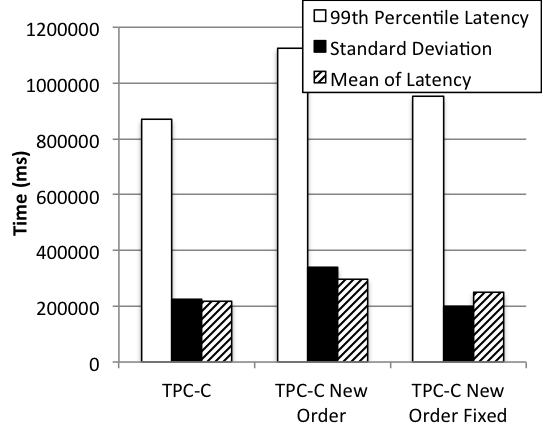
\includegraphics[scale=0.7]{plots/mysql-var}
\caption{99th percentile, standard deviation and average latency in MySQL}
\label{fig:mysql-var}
\end{figure}

\begin{figure}[h]
\centering
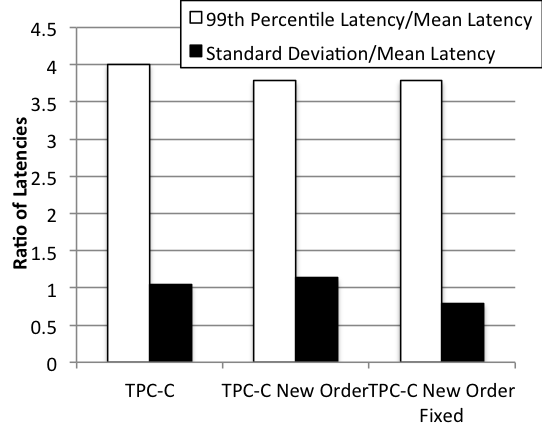
\includegraphics[scale=0.7]{plots/mysql-ratio}
\caption{99th percentile and standard deviation are several folds larger than
the average latency in MySQL}
\label{fig:mysql-ratio}
\end{figure}

As can be seen from figure \ref{fig:mysql-ratio}, the standard deviation of
transaction latencies is almost 3 times of the average latency. On the other 
hand, 99th percentile is a lot worse than standard deviation because no matter
which benchmark we use, the 99th percentile latency is an order of magnitude
larger then the average latency.

